%% SW design: Applikationsmodeller

Selve designet af softwaren bygger på de følgende applikationsmodeller. Her laves der sekvens- og klassediagrammer over hver del af systemet samt klassebeskrivelser hvor funktionen for de enkelte metoder beskrives.

\subsection{Master}
Applikationsmodeller for Master.

\begin{figure}[htbp] \centering
{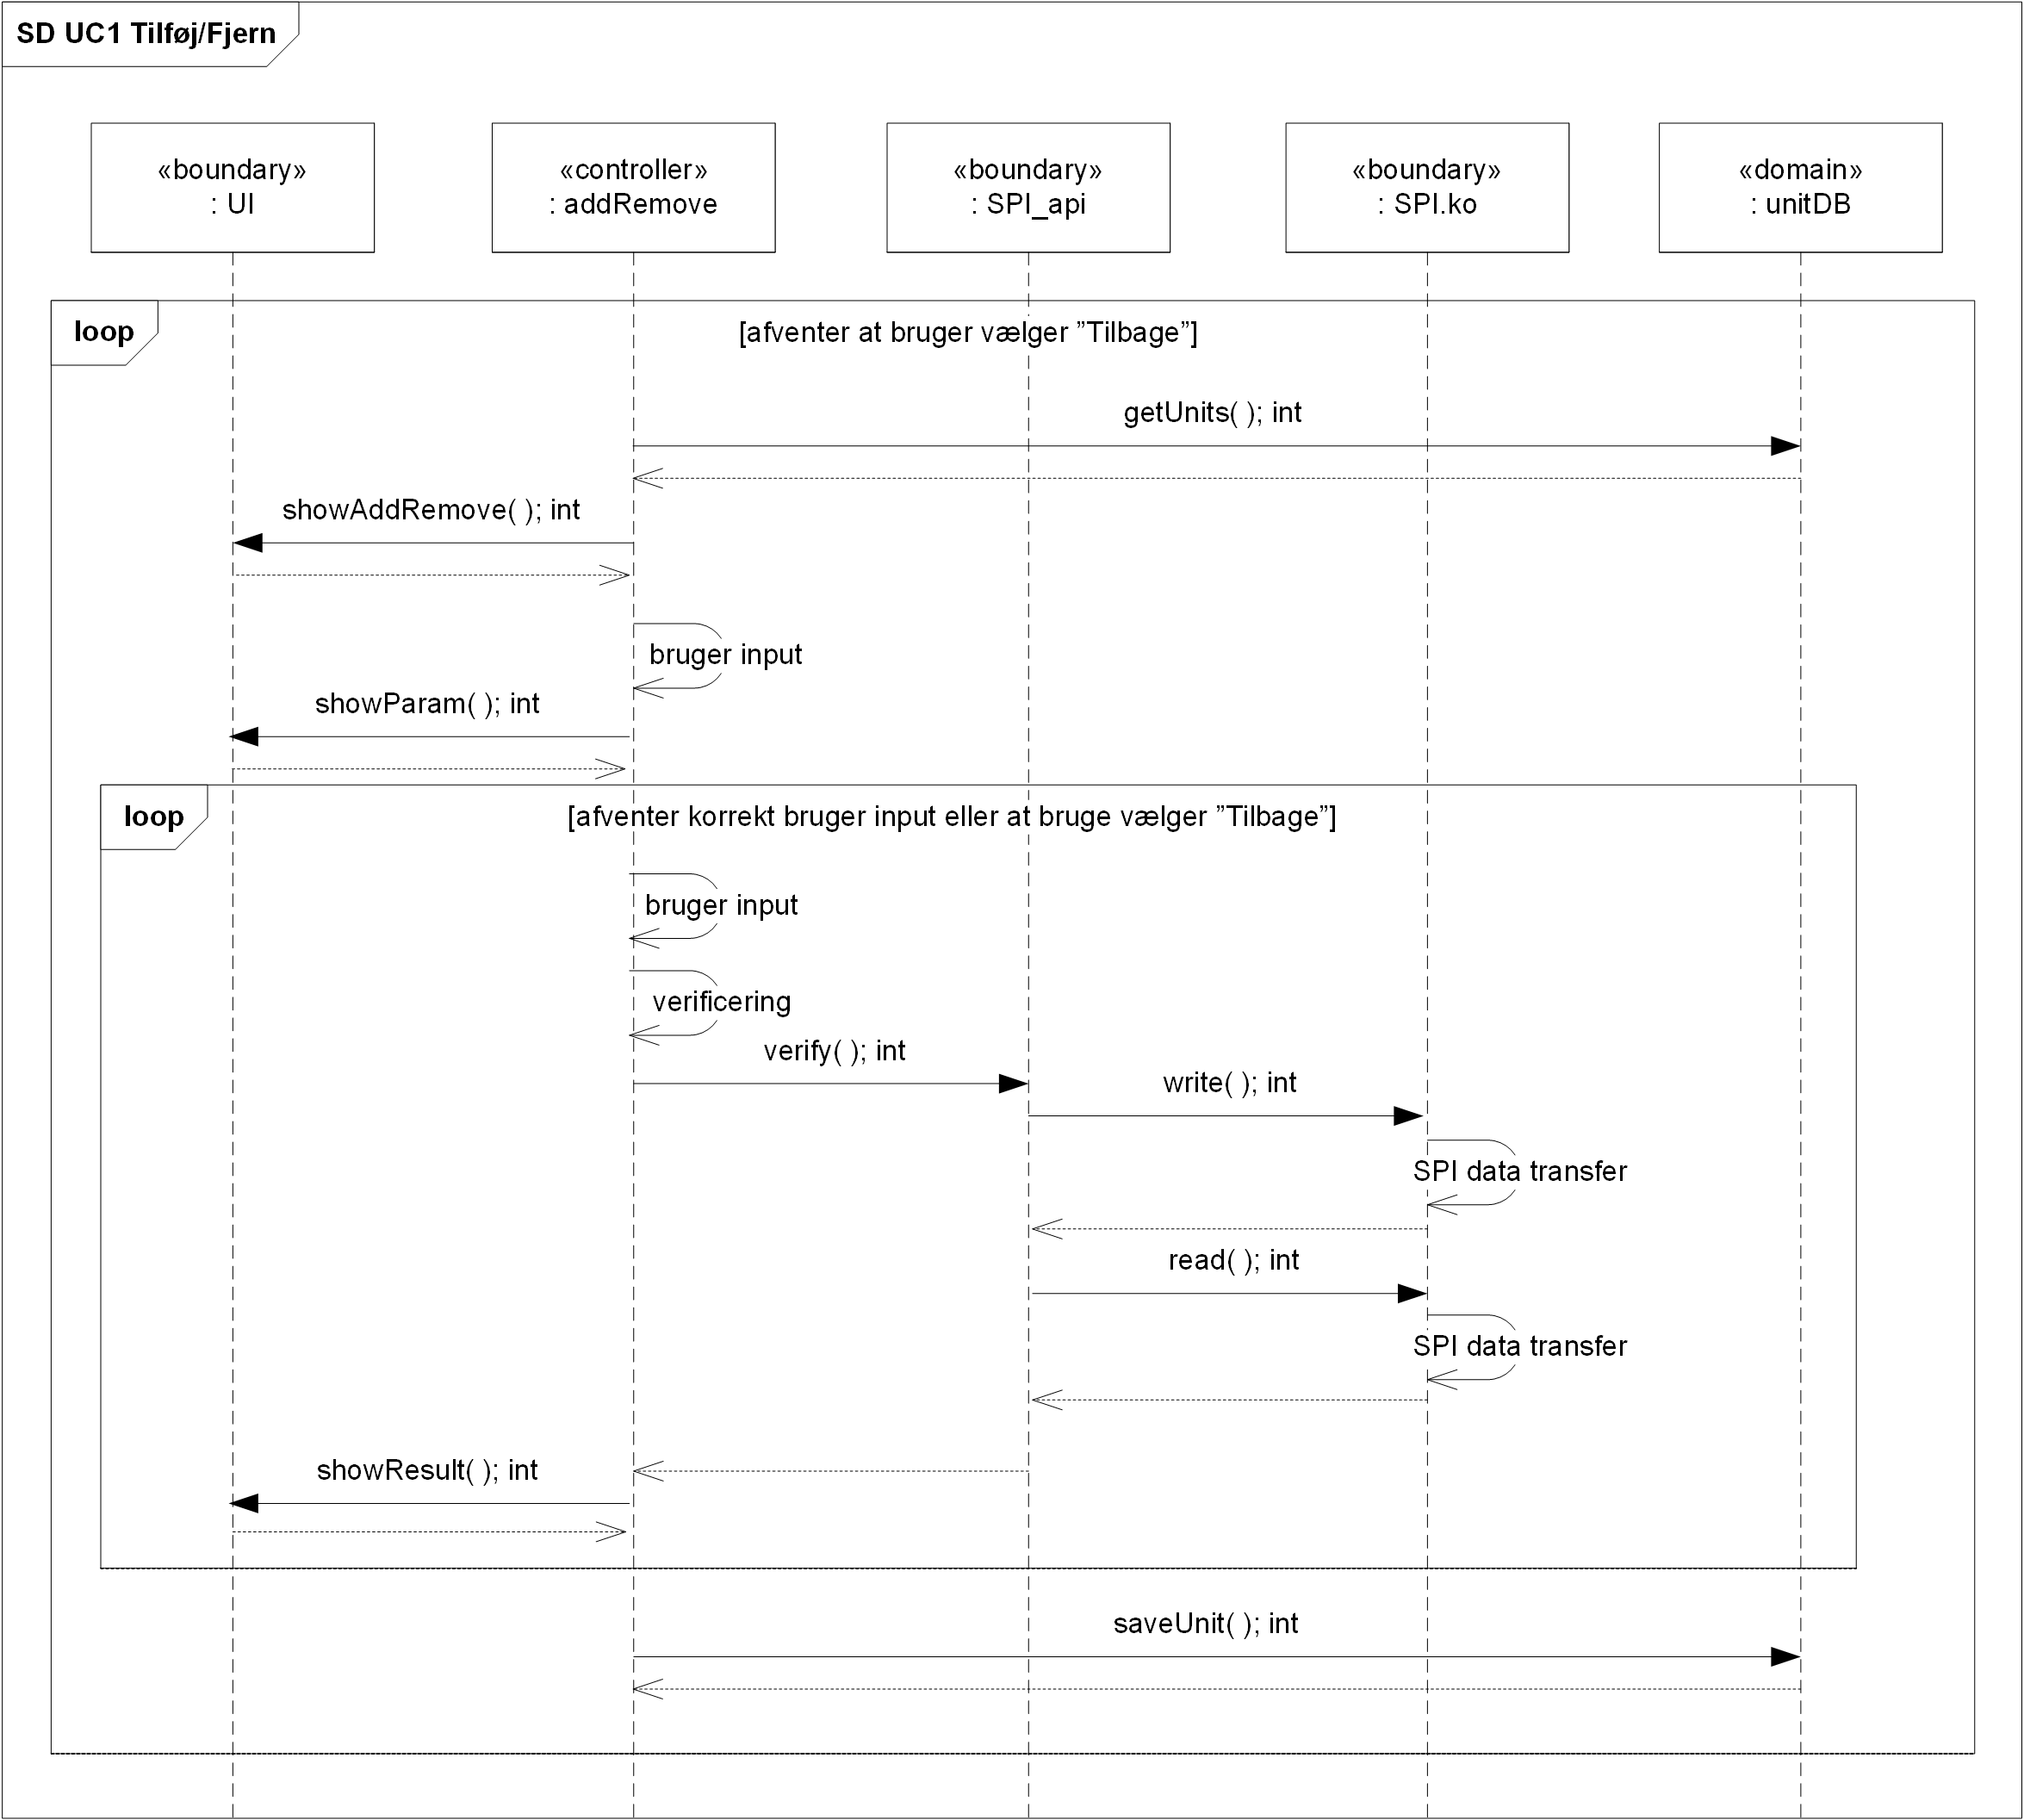
\includegraphics[scale=0.8]{filer/design/a_uc1}}
\caption{Sekvensdiagram UC1}
\label{fig:Sekvensdiagram UC1}
\end{figure} 

\begin{figure}[htbp] \centering
{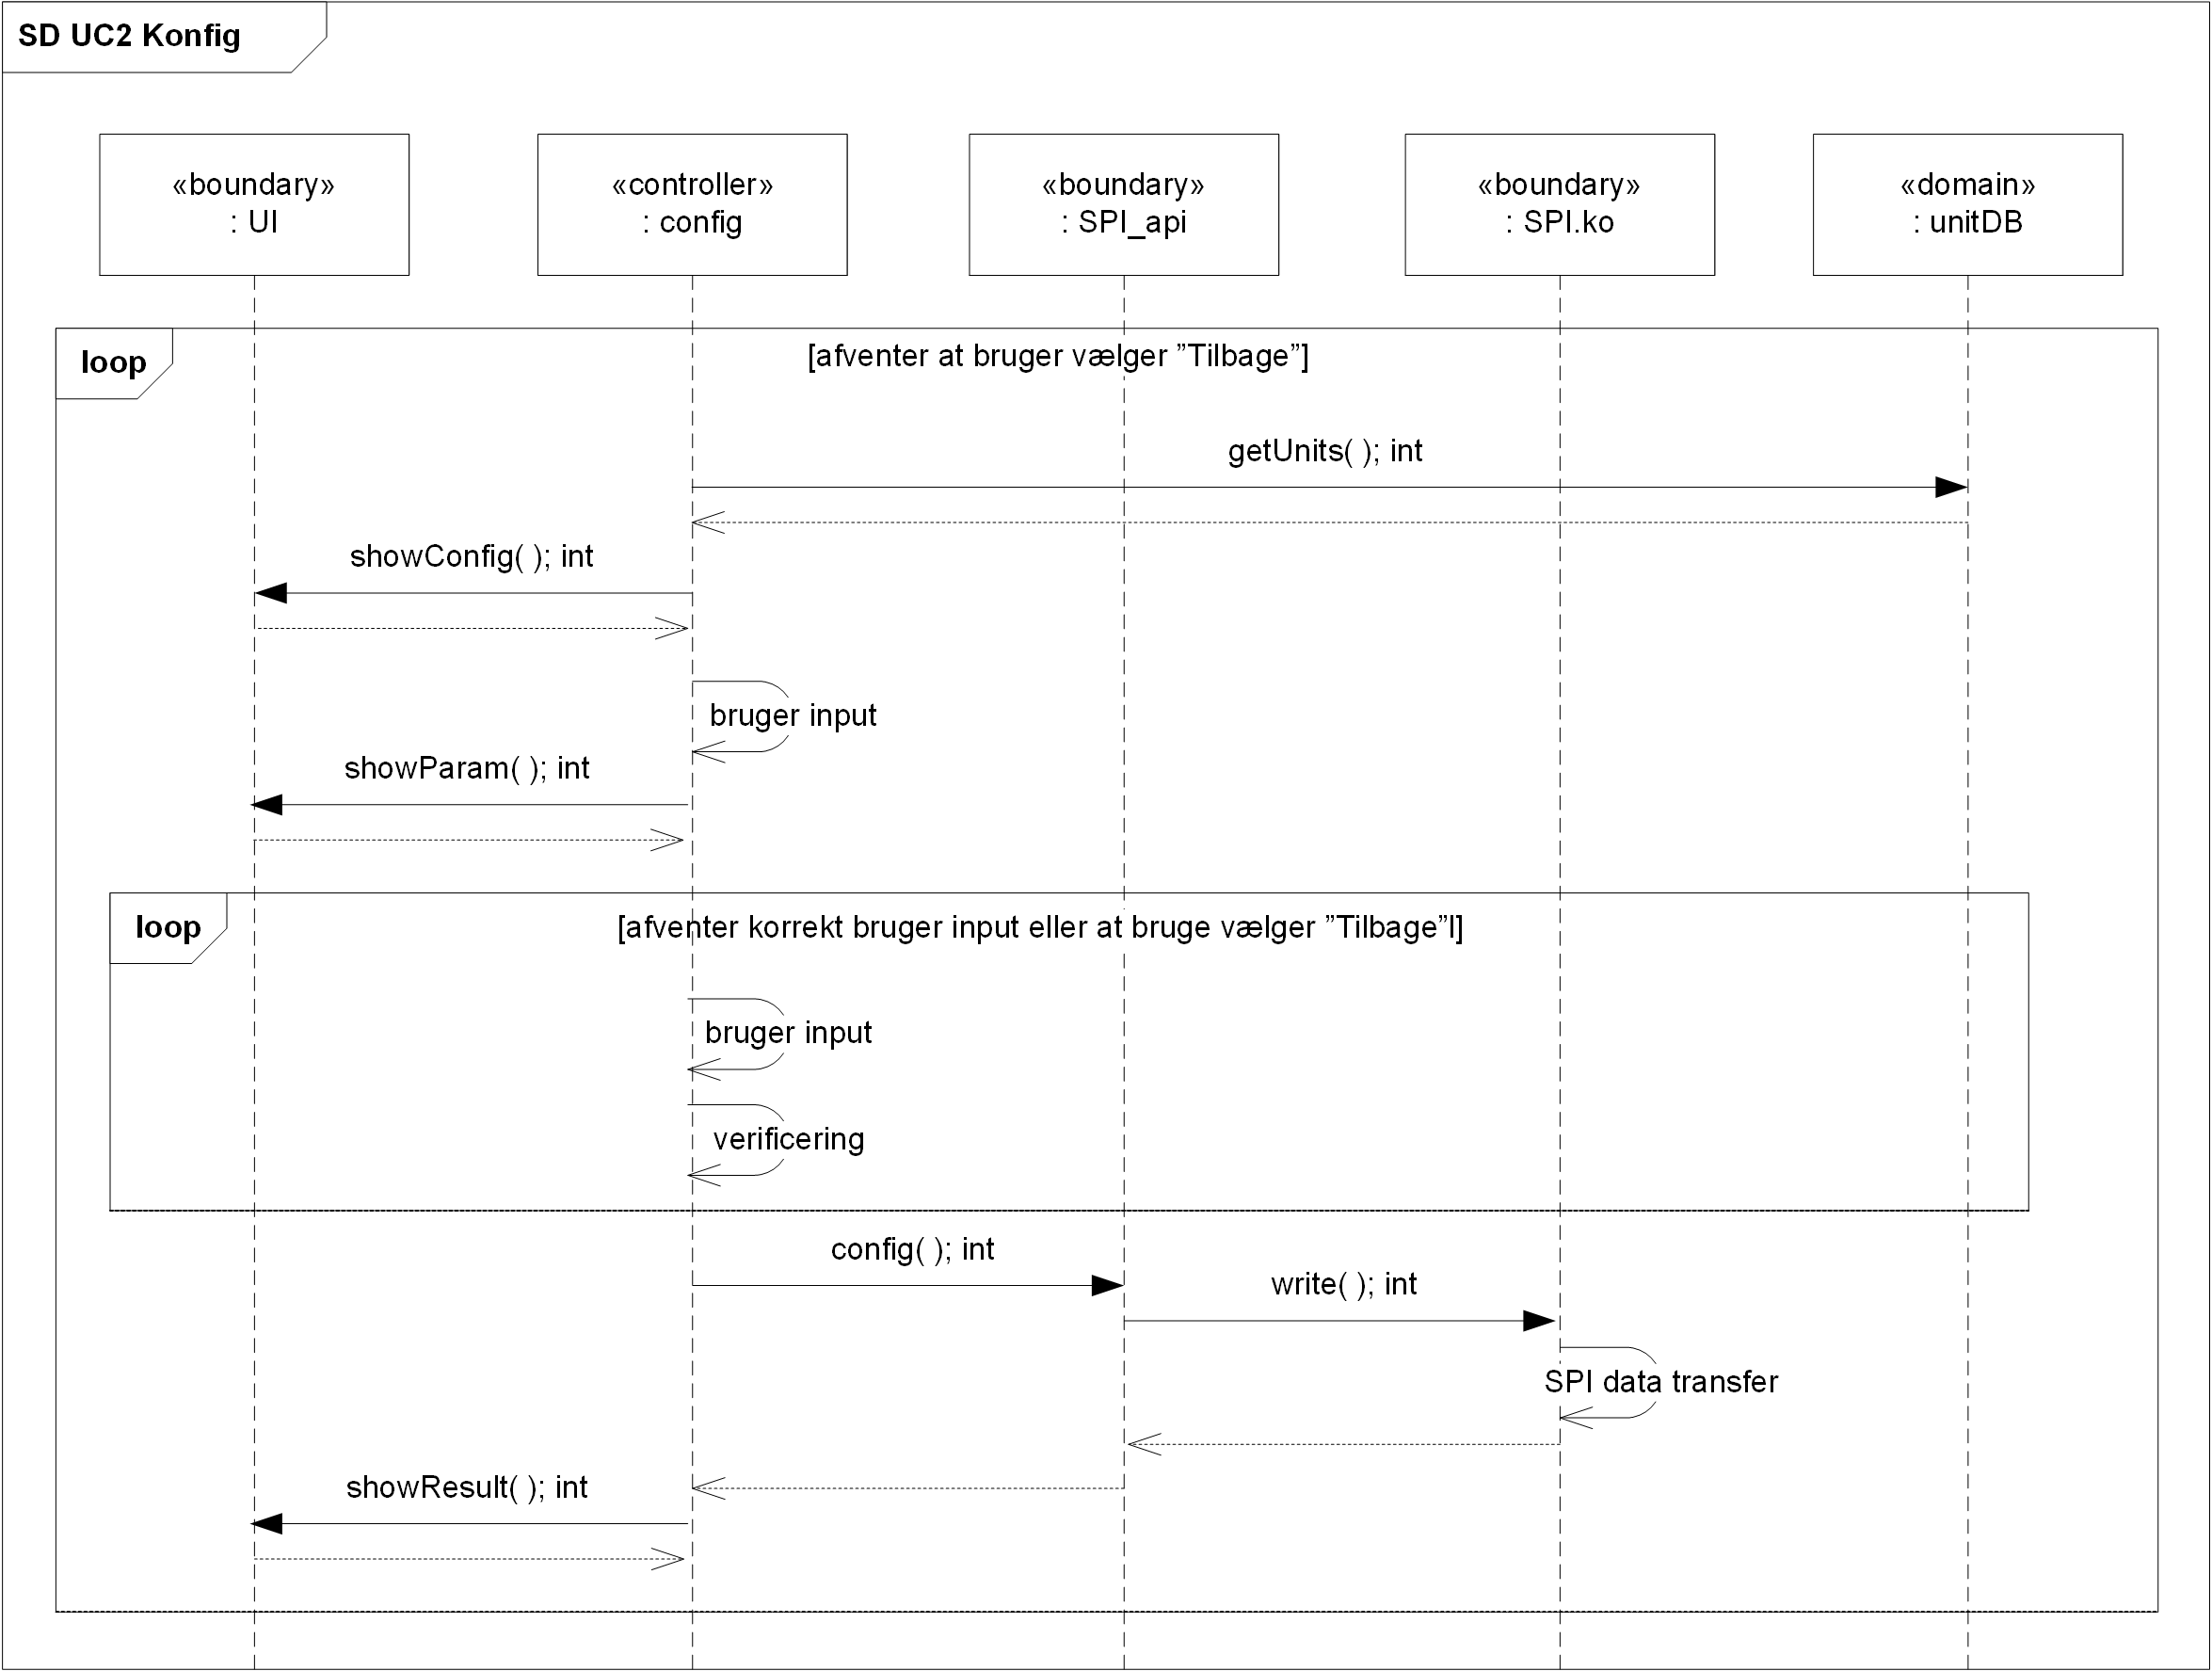
\includegraphics[scale=0.8]{filer/design/a_uc2}}
\caption{Sekvensdiagram UC2}
\label{fig:Sekvensdiagram UC2}
\end{figure} 

\begin{figure}[htbp] \centering
{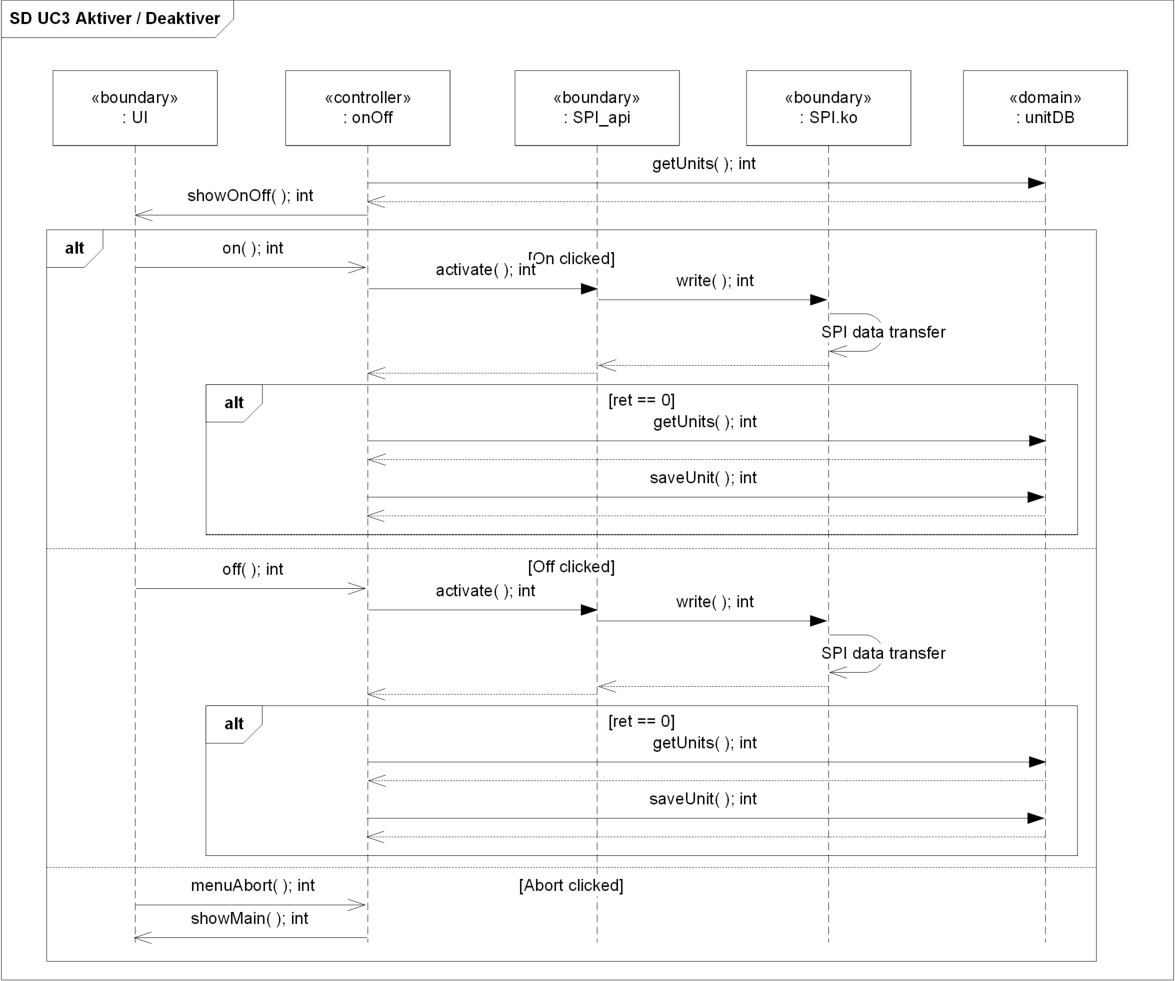
\includegraphics[scale=0.8]{filer/design/a_uc3}}
\caption{Sekvensdiagram UC3}
\label{fig:Sekvensdiagram UC3}
\end{figure} 

\begin{figure}[htbp] \centering
{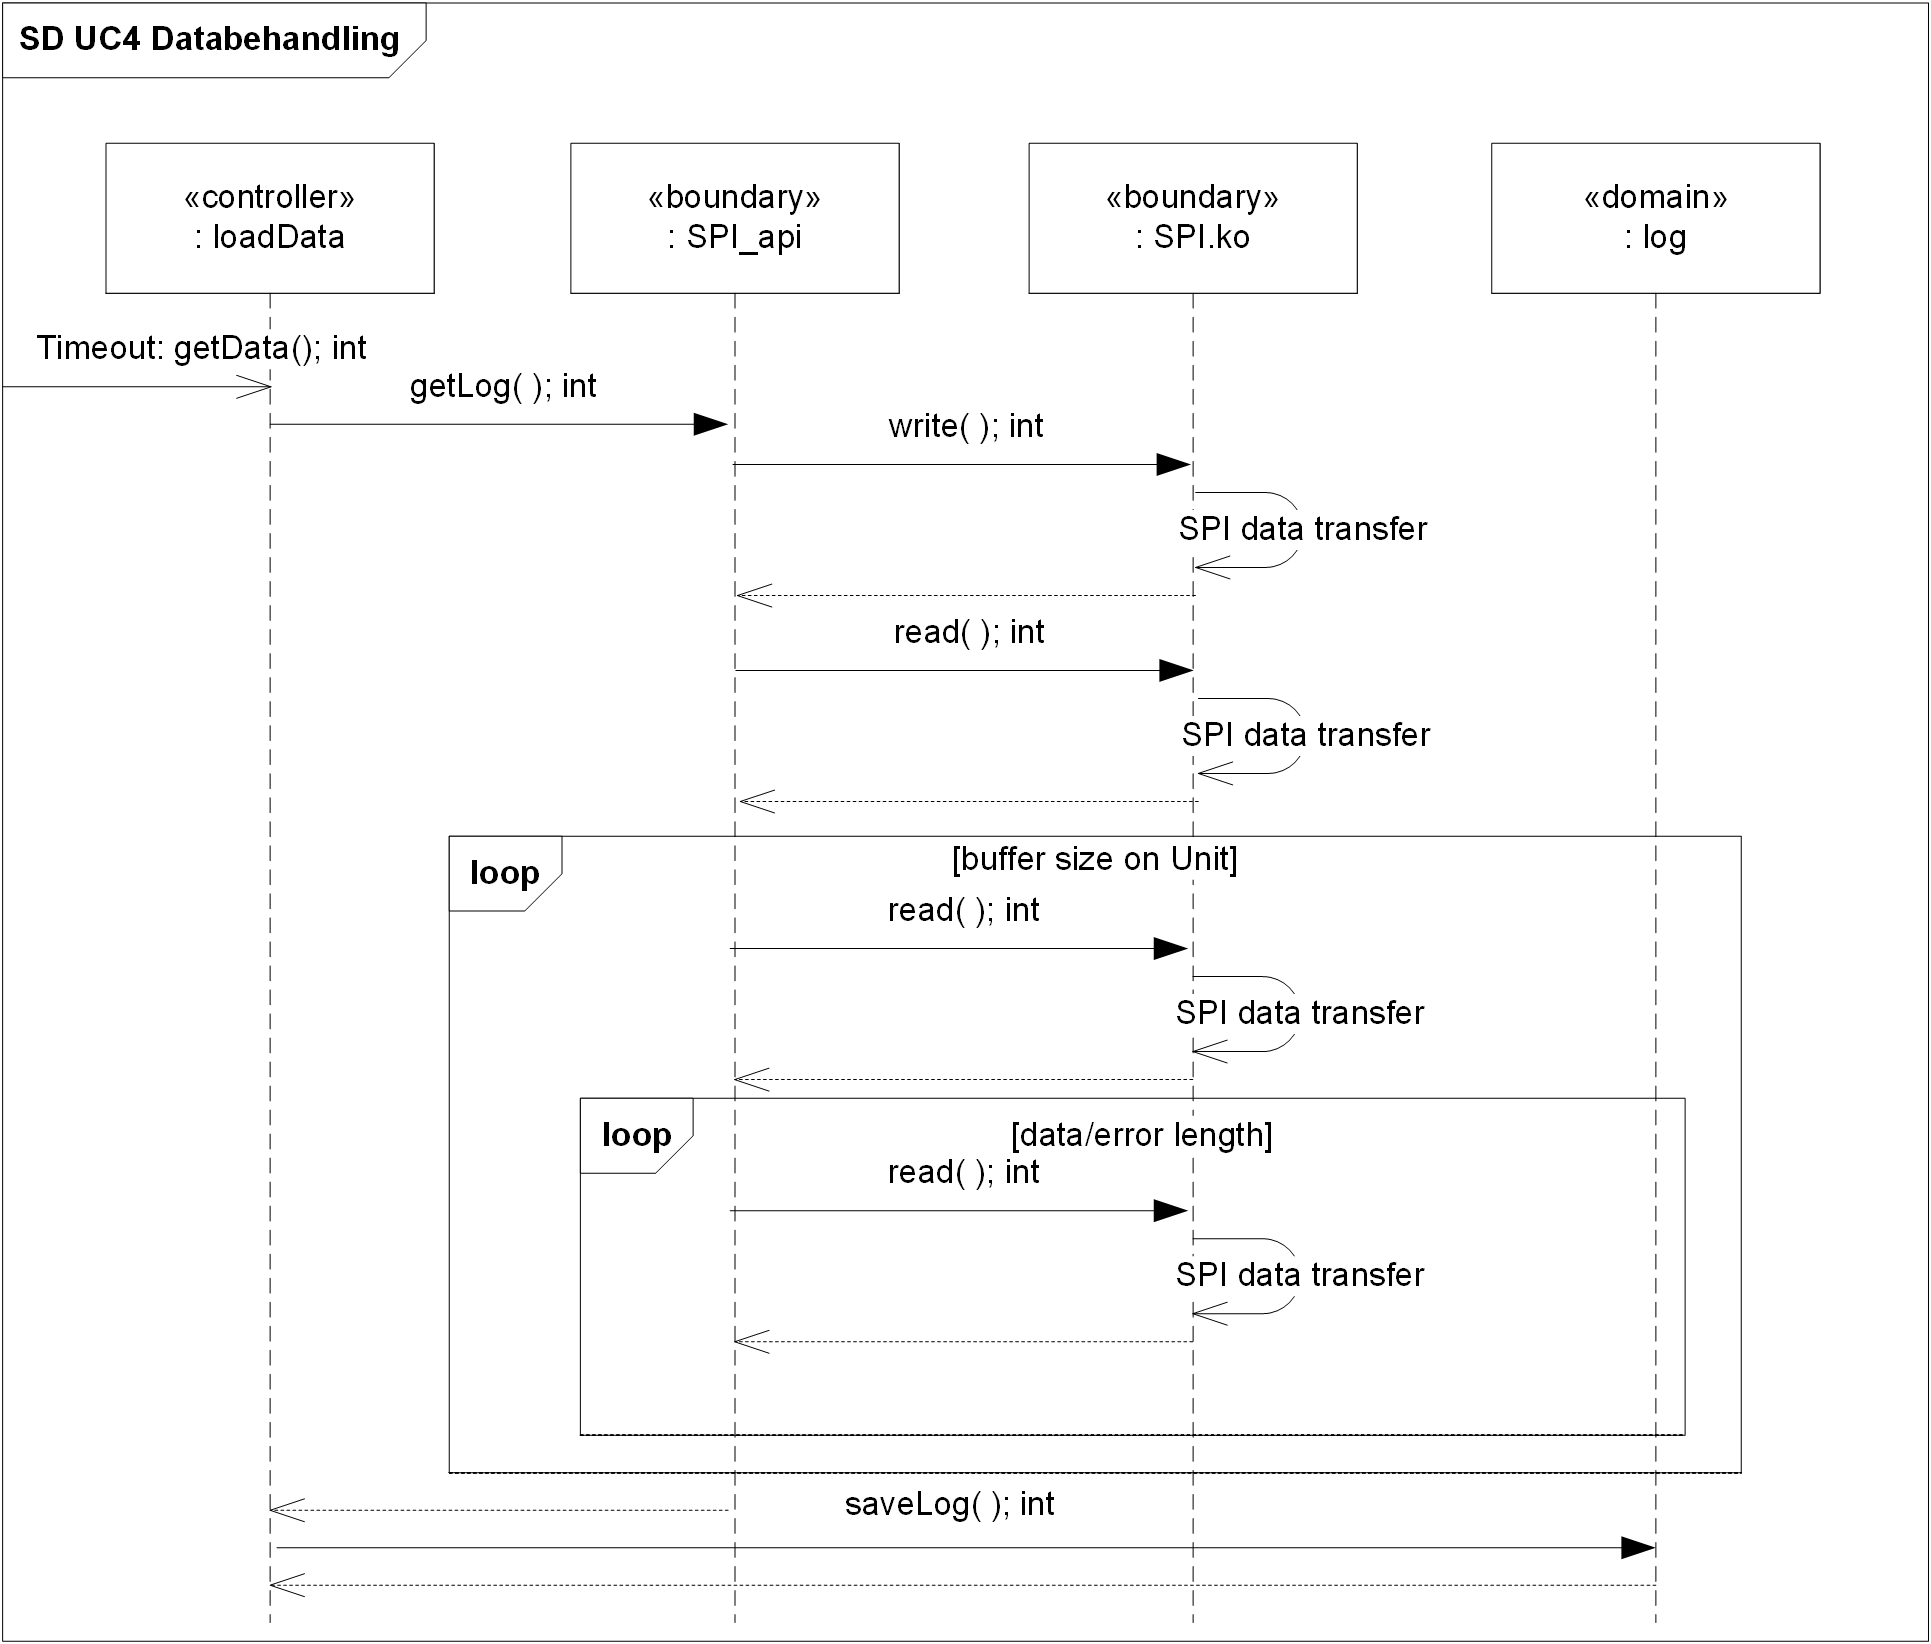
\includegraphics[scale=0.8]{filer/design/a_uc4}}
\caption{Sekvensdiagram UC4}
\label{fig:Sekvensdiagram UC4}
\end{figure} 

\begin{figure}[htbp] \centering
{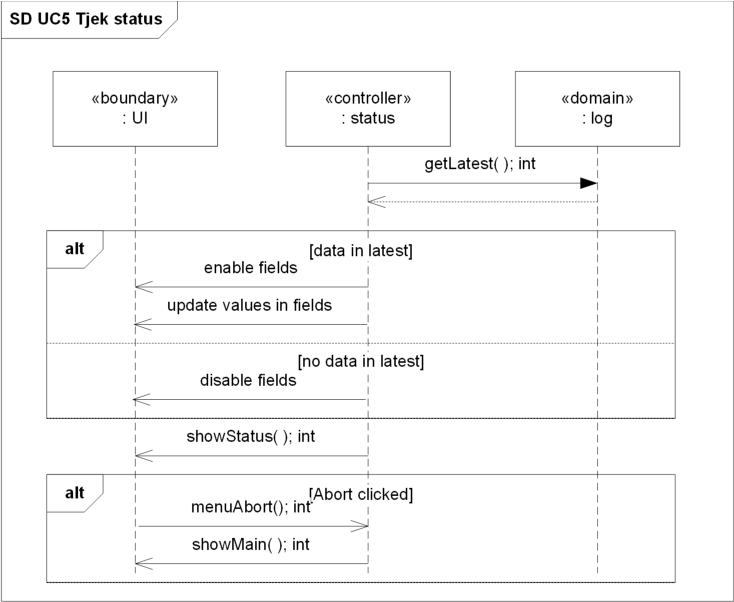
\includegraphics[scale=1]{filer/design/a_uc5}}
\caption{Sekvensdiagram UC5}
\label{fig:Sekvensdiagram UC5}
\end{figure} 

\begin{figure}[htbp] \centering
{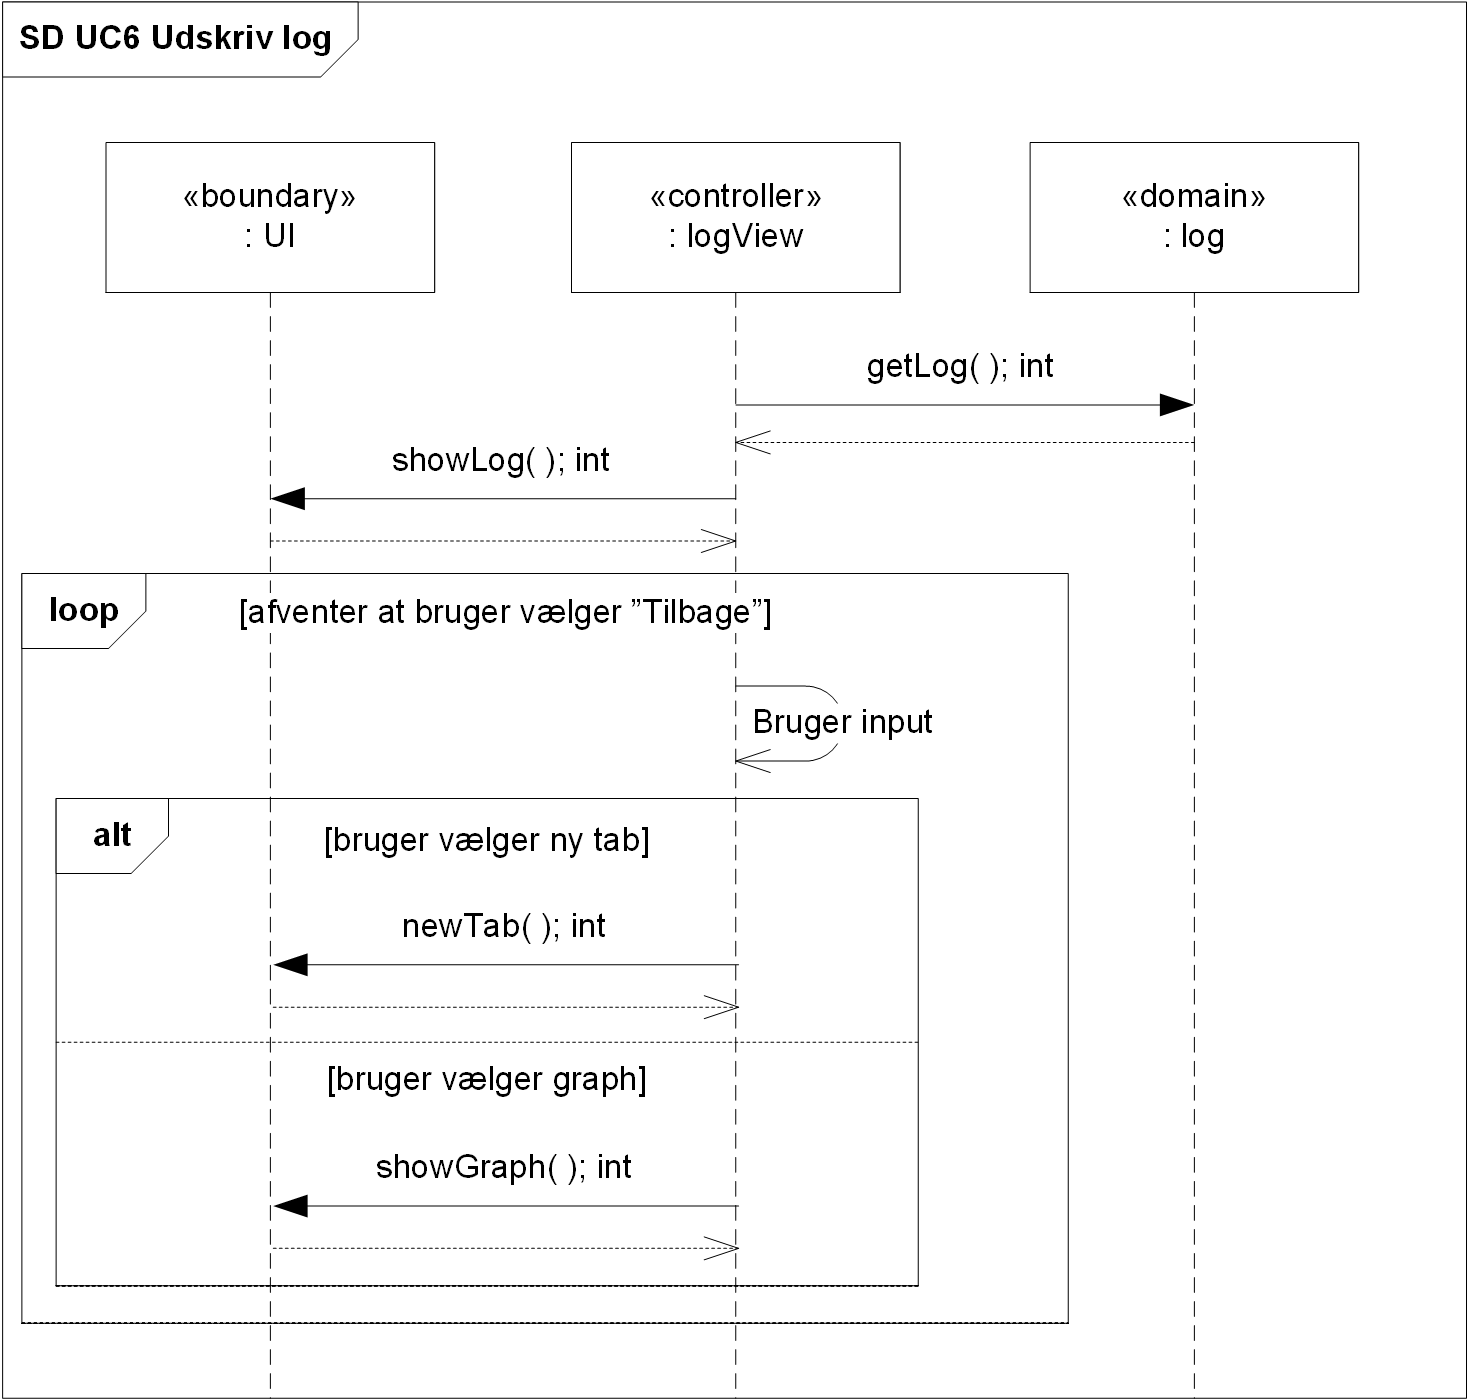
\includegraphics[scale=1]{filer/design/a_uc6}}
\caption{Sekvensdiagram UC6}
\label{fig:Sekvensdiagram UC6}
\end{figure} 

\clearpage
\begin{figure}[htbp] \centering
{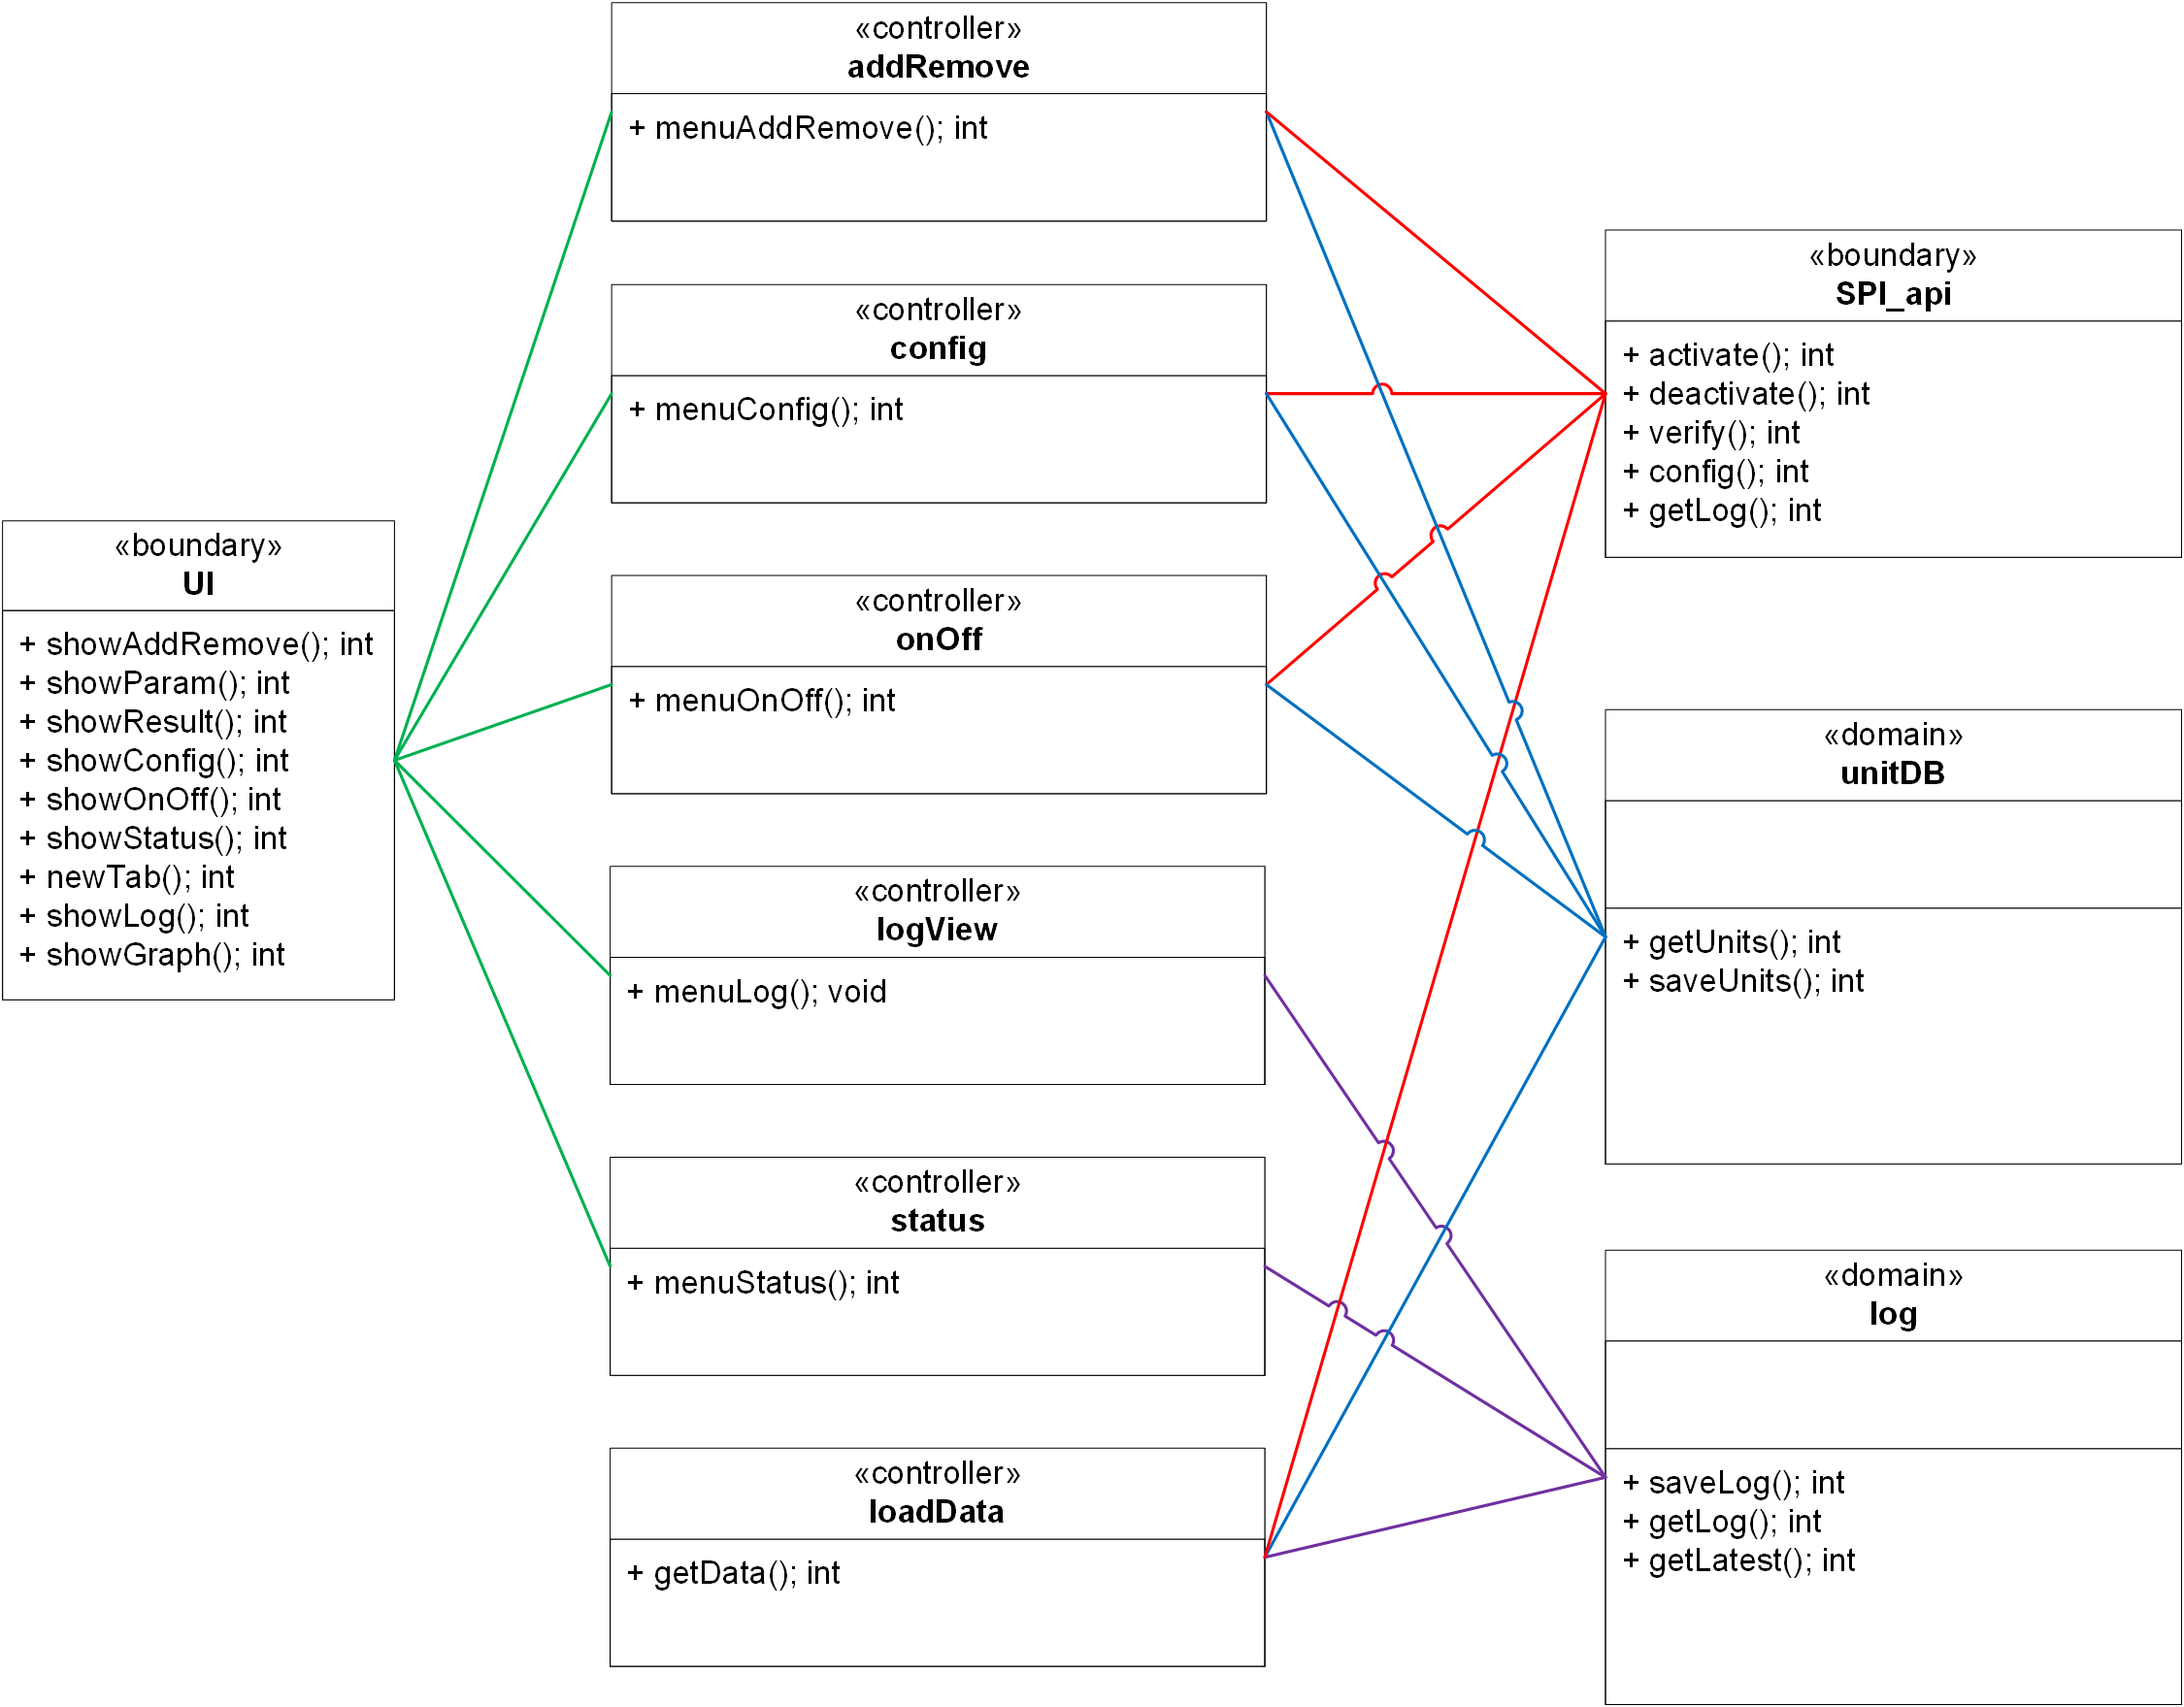
\includegraphics[width=\textwidth]{filer/design/sw_class_devkit}}
\caption{Klassediagram for Master (Devkit8000)}
\label{fig:klassediagram devkit8000}
\end{figure} 

Efter udarbejdelsen af sekvensdiagrammer samles alle metode kald mellem klasserne til et klassediagram som ses ovenfor på figur \ref{fig:klassediagram devkit8000}. Efter dette klassediagram udarbejdes en klassebeskrivelse hvor der tænkes over hvilke attributter de forskellige metoder skal have for at kunne udføre deres ansvar. Det bliver så fulgt op med et endeligt statisk klassediagram som inkluderer alle attributter og metoder.

\clearpage
\subsection{Enhed}
Applikationsmodeller for Enhed.

\begin{figure}[htbp] \centering
{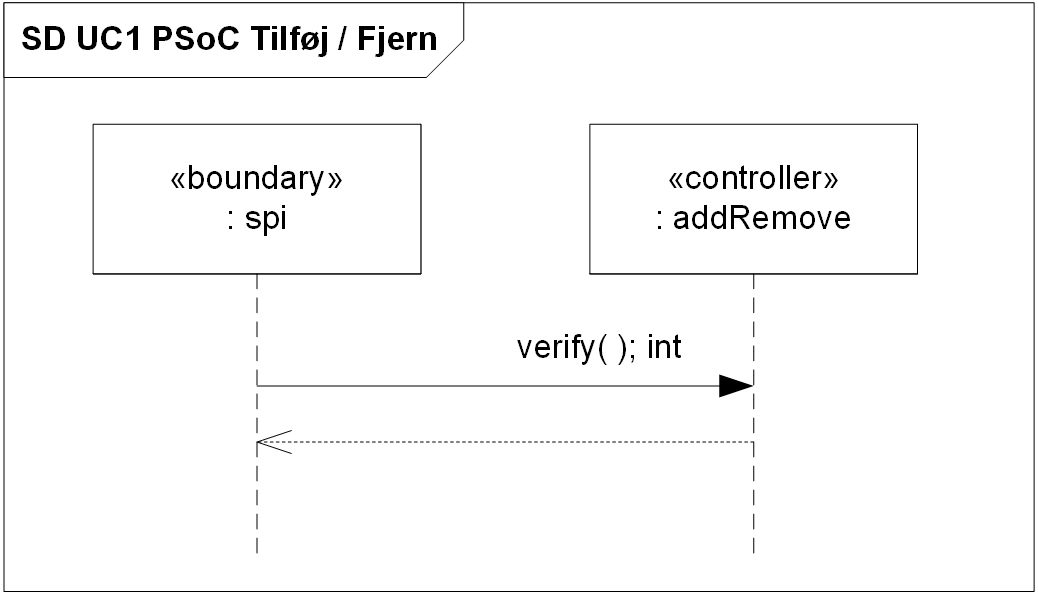
\includegraphics[scale=1]{filer/design/a_psoc_uc1}}
\caption{Sekvensdiagram UC1}
\label{fig:psoc_sd_uc1}
\end{figure} 

\begin{figure}[htbp] \centering
{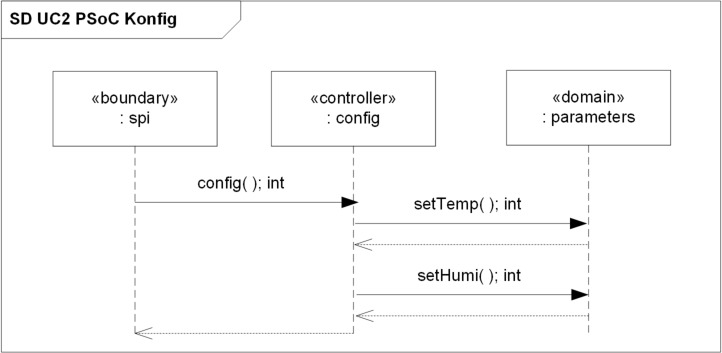
\includegraphics[scale=1]{filer/design/a_psoc_uc2}}
\caption{Sekvensdiagram UC2}
\label{fig:psoc_sd_uc2}
\end{figure} 

\begin{figure}[htbp] \centering
{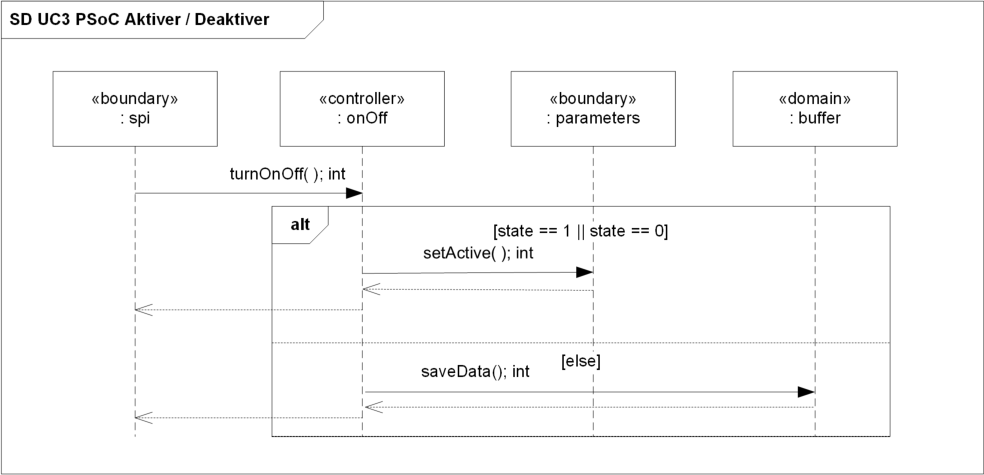
\includegraphics[scale=1]{filer/design/a_psoc_uc3}}
\caption{Sekvensdiagram UC3}
\label{fig:psoc_sd_uc3}
\end{figure} 

\begin{figure}[htbp] \centering
{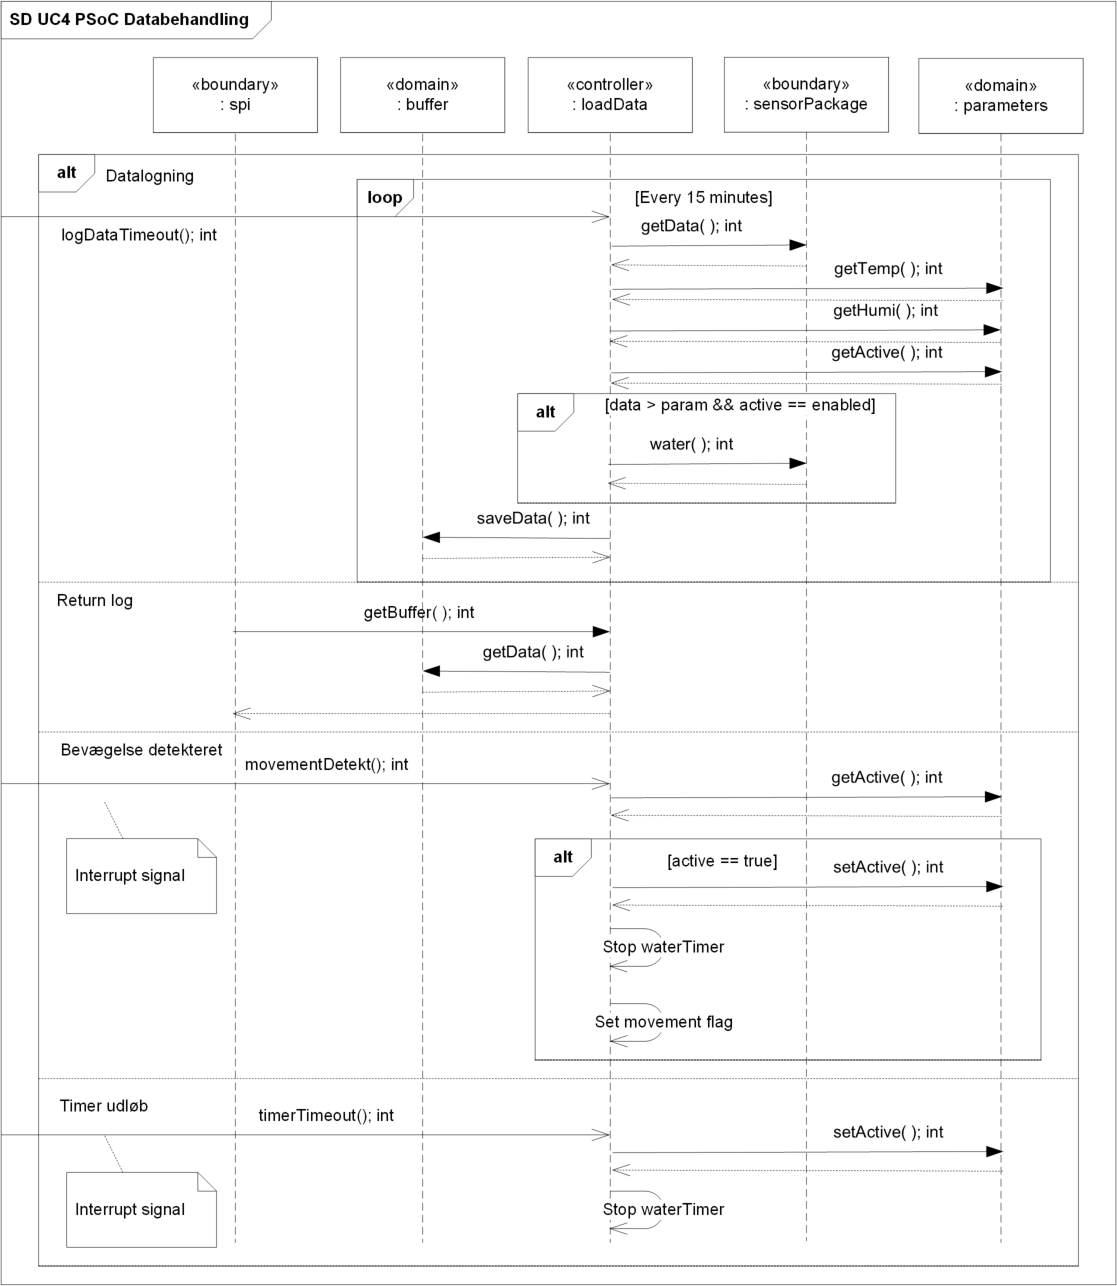
\includegraphics[scale=0.8]{filer/design/a_psoc_uc4}}
\caption{Sekvensdiagram UC4}
\label{fig:psoc_sd_uc4}
\end{figure} 

\clearpage
Ovenstående sekvensdiagrammer ender også ud i et statisk klassediagram. Det er vist på figur \ref{fig:psoc_klassediagram}.

\begin{figure}[htbp] \centering
{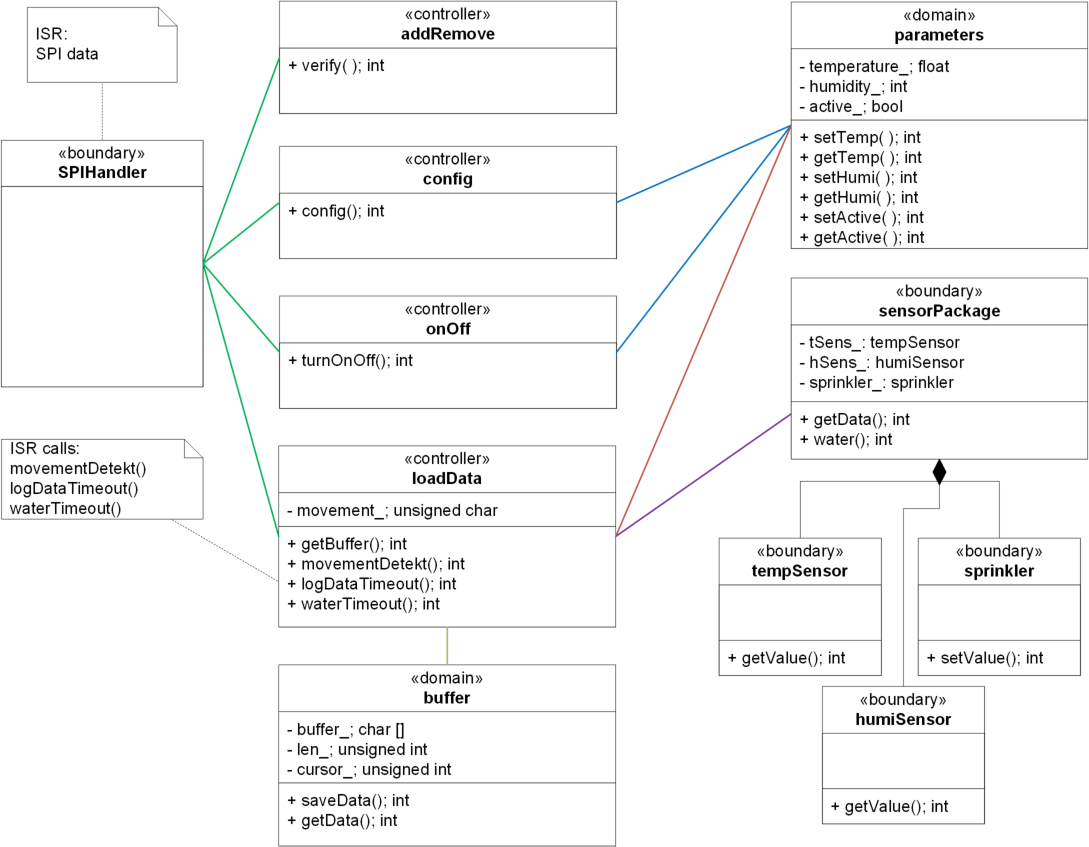
\includegraphics[width=\textwidth]{filer/design/sw_class_psoc}}
\caption{Klassediagram for Enhed (PSoC)}
\label{fig:psoc_klassediagram}
\end{figure} 